 %% bare_conf.tex
%% V1.4b
%% 2015/08/26
%% by Michael Shell
%% See:
%% http://www.michaelshell.org/
%% for current contact information.
%%
%% This is a skeleton file demonstrating the use of IEEEtran.cls
%% (requires IEEEtran.cls version 1.8b or later) with an IEEE
%% conference paper.
%%
%% Support sites:
%% http://www.michaelshell.org/tex/ieeetran/
%% http://www.ctan.org/pkg/ieeetran
%% and
%% http://www.ieee.org/

%\documentclass[conference,specification,annotation,times]{IEEEtran}
\documentclass[runningheads]{llncs}

\usepackage[T1]{fontenc}
\usepackage{graphicx}
\usepackage{soul}
\usepackage[normalem]{ulem}
\usepackage{comment}
\usepackage{xcolor}
\usepackage{listings}
\usepackage{tabularx}
\newcommand{\PreserveBackslash}[1]{\let\temp=\\#1\let\\=\temp}
\newcolumntype{C}[1]{>{\PreserveBackslash\centering}p{#1}}
\newcolumntype{R}[1]{>{\PreserveBackslash\raggedleft}p{#1}}
\newcolumntype{L}[1]{>{\PreserveBackslash\raggedright}p{#1}}
\definecolor{cred}{HTML}{FFB6B3}
\definecolor{cyellow}{HTML}{F7F4BA}
\definecolor{cgreen}{HTML}{E2F7DF}
\newcommand{\supported}{{\cellcolor{cgreen} $+$}}
\newcommand{\partially}{{\cellcolor{cyellow} $+/-$}}
\newcommand{\unsupported}{{\cellcolor{cred} $-$}}
\newcommand{\ra}{{\rightarrow}}
\newcommand{\etal}{\it et al. \normalfont}

%\newif\ifcomments
% comment out a different line to toggle comments
%\commentstrue
% \commentsfalse
\newcommand{\commentColor}[3]{\textcolor{#3}{[\textbf{#1:} #2]}}
\newcommand{\commentPO}[1]{\commentColor{PO}{#1}{teal}}
\newcommand{\commentVV}[1]{\commentColor{VV}{#1}{orange}}

\newcommand{\PO}[1]{\textcolor{teal}{#1}}
\newcommand{\VV}[1]{\textcolor{orange}{#1}}

\newcommand{\soutVV}[1]{\VV{\st{#1}}}
\newcommand{\corrPO}[2]{\soutPO{#1} \PO{#2}}
\newcommand{\N}{{\mathbb N}}
\newcommand{\NN}{\mathcal N}

% *** MISC UTILITY PACKAGES ***
%
%\usepackage{ifpdf}
% Heiko Oberdiek's ifpdf.sty is very useful if you need conditional
% compilation based on whether the output is pdf or dvi.
% usage:
% \ifpdf
%   % pdf code
% \else
%   % dvi code
% \fi

% *** CITATION PACKAGES ***
%
\usepackage{cite}

% *** GRAPHICS RELATED PACKAGES ***
%
% \ifCLASSINFOpdf
  \usepackage[pdftex]{graphicx}
  % declare the path(s) where your graphic files are
   \graphicspath{{./images}}
  % and their extensions so you won't have to specify these with
  % every instance of \includegraphics
   \DeclareGraphicsExtensions{.pdf,.jpeg,.png}
% \else
  % or other class option (dvipsone, dvipdf, if not using dvips). graphicx
  % will default to the driver specified in the system graphics.cfg if no
  % driver is specified.
%   \usepackage[dvips]{graphicx}
  % declare the path(s) where your graphic files are
  % \graphicspath{{../eps/}}
  % and their extensions so you won't have to specify these with
  % every instance of \includegraphics
  % \DeclareGraphicsExtensions{.eps}
% \fi
\usepackage{subcaption}
\usepackage{caption}
\usepackage{icomma}
\usepackage{xcolor}
\usepackage{array}

% *** MATH PACKAGES ***
%
\usepackage{amsmath}

% *** SPECIALIZED LIST PACKAGES ***
%
% \usepackage{algorithm}
\usepackage[ruled,linesnumbered,vlined]{algorithm2e}
\newcommand\mycommfont[1]{\rmfamily{#1}}
\SetCommentSty{mycommfont}
% \usepackage{algorithmic}



% *** ALIGNMENT PACKAGES ***
%
%\usepackage{array}


% IEEEtran contains the IEEEeqnarray family of commands that can be used to
% generate multiline equations as well as matrices, tables, etc., of high
% quality.




% *** SUBFIGURE PACKAGES ***
%\ifCLASSOPTIONcompsoc
%  \usepackage[caption=false,font=normalsize,labelfont=sf,textfont=sf]{subfig}
%\else
%  \usepackage[caption=false,font=footnotesize]{subfig}
%\fi


% *** FLOAT PACKAGES ***
%
%\usepackage{fixltx2e}
%\usepackage{stfloats}
% \usepackage{dblfloatfix}


% *** PDF, URL AND HYPERLINK PACKAGES ***
%
%\usepackage{url}


% *** Do not adjust lengths that control margins, column widths, etc. ***
% *** Do not use packages that alter fonts (such as pslatex).         ***
% There should be no need to do such things with IEEEtran.cls V1.6 and later.
% (Unless specifically asked to do so by the journal or conference you plan
% to submit to, of course. )


% correct bad hyphenation here
\hyphenation{op-tical net-works semi-conduc-tor}


\begin{document}
%
% paper title
% Titles are generally capitalized except for words such as a, an, and, as,
% at, but, by, for, in, nor, of, on, or, the, to and up, which are usually
% not capitalized unless they are the first or last word of the title.
% Linebreaks \\can be used within to get better formatting as desired.
% Do not put math or special symbols in the title.
%\title{Automatic conversion and testing of\\IEC~61131-3 systems to IEC~61499 systems}

\title{Formal Modelling, Analysis, and Synthesis of Modular Industrial Systems inspired by Net Condition/Event Systems }

\author{
Midhun Xavier\inst{1} \orcidID{0000-0003-3371-6075}  \and
Sandeep Patil\inst{1} \orcidID{0000-0003-2936-4185}  \and
Victor Dubinin\inst{2} \orcidID{0000-0002-5761-2249}  \and
Valeriy Vyatkin\inst{1,3} \orcidID{0000-0002-9315-9920} 
}
%
\authorrunning{V. Vyatkin \etal}
\titlerunning{Modular Industrial Systems Modelling}

% First names are abbreviated in the running head.
% If there are more than two authors, 'et al.' is used.
%
\institute{Department of Computer Science, \VV{Electrical} and Space Engineering, Luleå Tekniska Universitet, Sweden \email{midhun.xavier@ltu.se, sandeep.patil@ltu.se} \and
Independent researcher \email{dubinin.victor@gmail.com} \and Department of Electrical Engineering and Automation, Aalto University, Espoo, Finland
\email{vyatkin@ieee.org}}
%

% make the title area
\maketitle

% As a general rule, do not put math, special symbols or citations
% in the abstract
\begin{abstract}
   
This paper summarises recent developments in the application of modular formalisms to model-based verification of industrial automation systems. The paper is a tribute to the legacy of Professor Hans-Michael Hanisch who invented Net Condition/Event Systems (NCES) and passionately promoted the closed-loop modelling approach to modelling and analysis of automation systems. The paper surveys the related works and highlights the impact NCES has made on the current progress of modular automation systems verification.

\end{abstract}

% no keywords
\lstset{language=xml,
       basicstyle=\ttfamily\scriptsize
     }

\section{Introduction}
Modularity is a fundamental feature of technical systems, in particular in industrial automation and cyber-physical systems.
On the other hand, modular systems is a good example of distributed systems.
Petri nets (PN) have been known as a formal language specifically focused on modelling of distributed state systems. That suggests a clear overlap and the need to address modularity in formal modelling. Petri nets inspired an uncountable number of derivatives.

Modularity in the context of PN has been discussed for a long time. 
According to \cite{davidrajuh2019new}, the concept of Modular Petri Nets has been through four generations of development. 

On the other hand, the concept of Condition/Event Systems (C/ES)
 \cite{sreenivas1991condition} was invented to model modular systems composed of communicating modules and study their generic properties.

Net Condition/Event Systems (NCES) \cite{rausch1995net} is a particular case of C/ES where modules are defined as (extended) Petri nets. It was proposed to model more efficiently distributed systems that are modular. 

One should note that computational analysis of NCES is in general undecidable as shown by Starke and Hanisch \cite{starke1997analysis}. Nevertheless, the formalism fits very well with the emerging engineering concepts for CPS such as service-oriented architecture (SOA) and IEC 61499 function blocks due to the properly addressed event-driven semantics. The initial effort of NCES application to IEC 61499 modelling is summarised in \cite{hanisch2009one}.

In this paper, we attempt to observe the developments related to the modelling and analysis of distributed modular industrial automation systems from the particular perspective of how the modular derivatives of Petri nets influence them.

The rest of the paper is structured as follows. In Section \ref{sec:def} the necessary definitions of NCES are provided. It is followed by a brief illustration of some features NCES provide for modelling distributed modular systems in Section \ref{sec:ncesmod}. Section \ref{sec:61499} contains some observations of similarities between IEC 61499 and NCES. Section \ref{sec:survey} attempts to overview the related research works on the modelling of modular systems. The recently developed modelling framework for modular systems based on IEC 61499 and influenced by the Condition/Event Systems paradigm is described in Section \ref{sec:framework}. The paper is concluded with a short summary and outlook in Section \ref{sec:summary} and acknowledgements. 

\section{Some definitions}\label{sec:def}

Net Condition/Event Systems (NCES) is a finite state formalism that preserves the graphical notation and the non-interleaving semantics of Petri nets \cite{Petri62}, and extends them with a clear and concise notion of signal inputs and outputs. The formalism was introduced in \cite{RaHA95} \VV{in 1995} and has been used in dozens of applications, especially in embedded industrial automation systems. 

%\fgx{8}{module}{Graphical notation of a NCES module.}{CEN}

\begin {figure}
    \centering
    
\includegraphics [width = .5 \textwidth] {images/nces_module.jpg}
    \caption {Graphical notation of an NCES module.}
    \label {fig:nces}
\end {figure}

Given a place/transition net $N=(P,T,F,m_0)$, the
Net Condition/Event System (NCES) is defined as a tuple
$\NN=(N,\theta_N,\Psi_N, Gr)$, where $\theta_N$ is an internal
structure of signal arcs, $\Psi_N$ is an input/output structure,
and $Gr \subseteq T$ is a set of so-called "obliged" transitions that fire as soon as it is enabled.
Fig. \ref{fig:nces} shows an example of an NCES module. 
The structure $\Psi_N$ consists of
condition and event inputs and outputs ($ci,ei,eo,co$). The
structure $\theta_N$ is formed from two types of {\it signal}
arcs. Condition arcs lead from places and condition inputs to
transitions and condition outputs. They provide additional
enableness conditions of the recipient transitions. Event arcs
from transitions and event inputs to transitions and event
outputs provide one-sided synchronization of the recipient
transitions: the firing of the source transition forces the firing of the recipient if the latter is enabled by the marking and conditions.

The NCES modules can be interconnected by the condition and event arcs, forming thus distributed and hierarchical models \VV{as illustrated in Fig.\ref{fig:composition}}.
NCES having no inputs can be analyzed without any additional
information about its external environment.

\begin {figure}
    \centering
    
\includegraphics [width = .5 \textwidth] {images/composition.jpg}
    \caption {Composition of NCES modules.}
    \label {fig:composition}
\end {figure}

The semantics of NCES cover both asynchronous and synchronous behaviour (required to model plants and controllers respectively). NCES are supported by a family of model-developing and model-checking tools, such as a graphic editor, SESA and ViVe (\cite{vive}).

The state of an NCES module is completely determined by the
current marking $m: P \righarrow \N_0$ of places and values of
inputs. A state transition is determined by the subset $\tau
\subseteq T$ of simultaneously fired transitions, called {\it
step}. The transitions having no incoming event arcs are called
{\it spontaneous}, otherwise {\it forced}. The step fully determines the
values of the event outputs of the module. In the original NCES version the step is formed by
choosing some\footnote{This means the step in NCES is non-deterministic.} of the enabled spontaneous transitions, and all the enabled transitions forced by the transitions already included in the step. 

A state of NCES is fully described by the marking of all its places (in the timed version also by clocks). A transition step specifies a state transition. 
When used for system analysis, a set of all reachable states (complete or partial) 
of NCES model is generated and then analyzed.

For describing the execution model of function blocks we use a deterministic dialect 
of NCES and the modeling approach that guarantee certain properties of the models as follows: 
\begin{enumerate}
\item In the chosen dialect a step is formed from all enabled spontaneous transitions and all forced transitions;
\item The models are designed so that there is no conflicts (i.e. deficient marking in some places) leading to non-deterministic choice of some of the enabled transitions;
\item The models also guarantee bounded marking in all places.
\end{enumerate}


\section{Modelling distributed systems with NCES}\label{sec:ncesmod}

To illustrate the key features of NCES modelling for distributed systems, let us consider an example of a simple distributed control system. In the system of two cylinders in Fig. \ref{fig:two_cylinders} each cylinder pushes a workpiece to the destination hole. The process starts when the workpiece appears in front of the corresponding cylinder as indicated by sensors P1 and P2 respectively. 
As it is clear from the Figure, cylinders can collide in the middle point, therefore the goal of controller design is to avoid such a situation. 


\begin {figure}
    \centering
    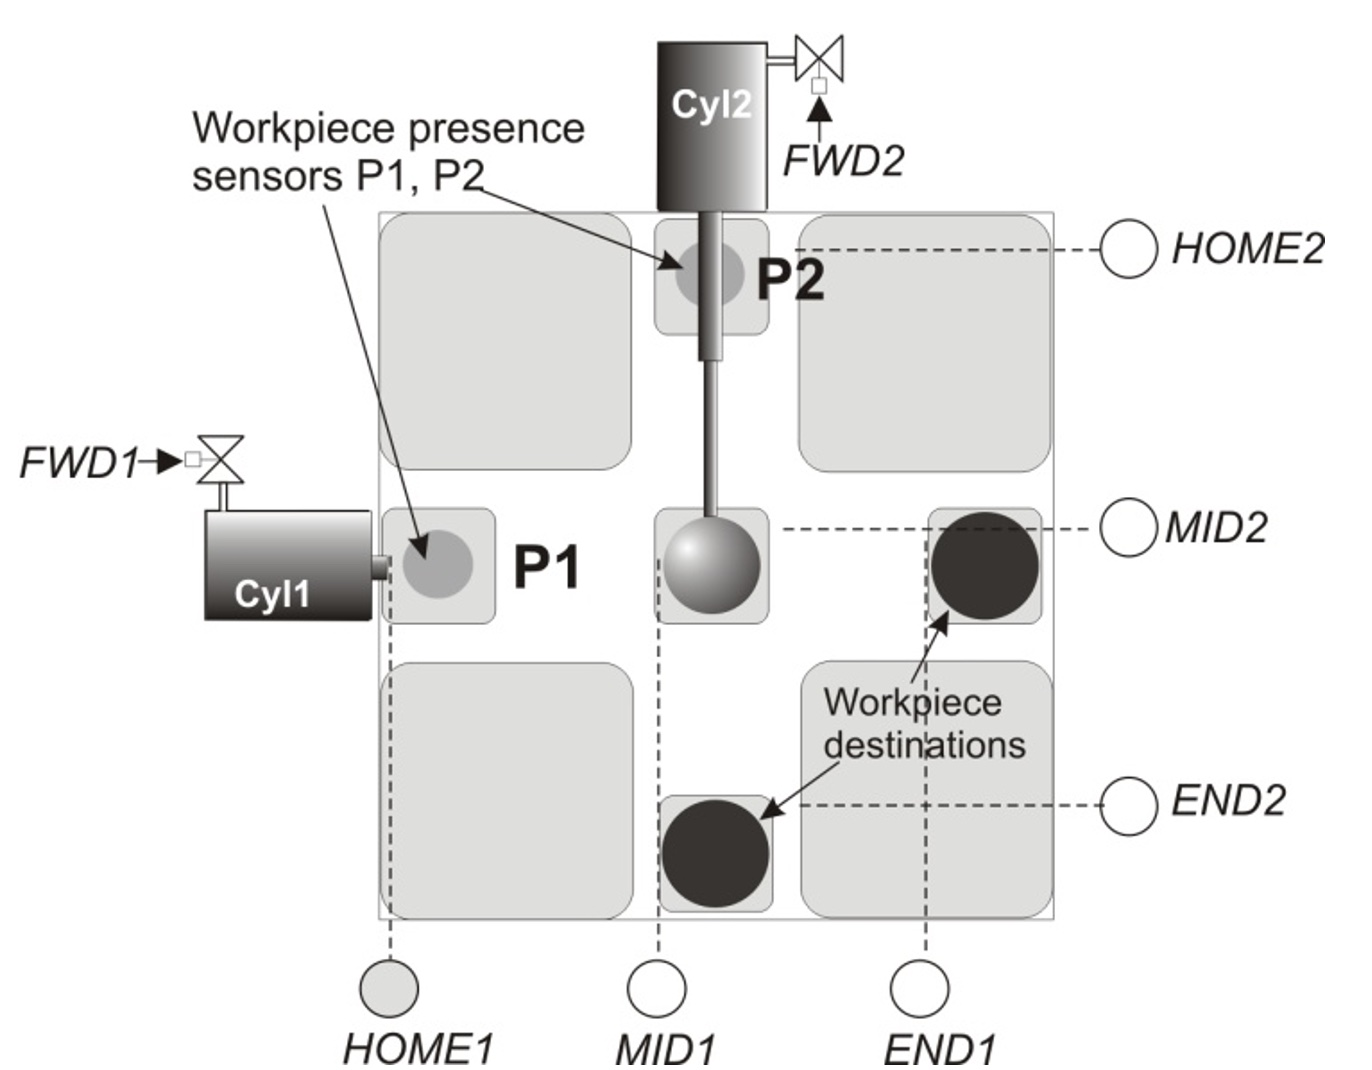
\includegraphics [width = .5 \textwidth] {images/two_cylinders.jpg}
    \caption {Two cylinders example of a distributed system.}
    \label {fig:two_cylinders}
\end {figure}

There are many possible ways to achieve the desired behaviour, which can be done by designing a “central” controller of both cylinders or a protocol ensuring that distributed controllers collaborate correctly. Distributed control is of interest for many practical reasons, for example for the case when control logic is “embedded” in each cylinder, so they can start working as soon as powered on.

\VV{NCES model of the two cylinders system with distributed control is presented in Fig. \ref{fig:nces_2_cyl}.}

\begin {figure}
    \centering
    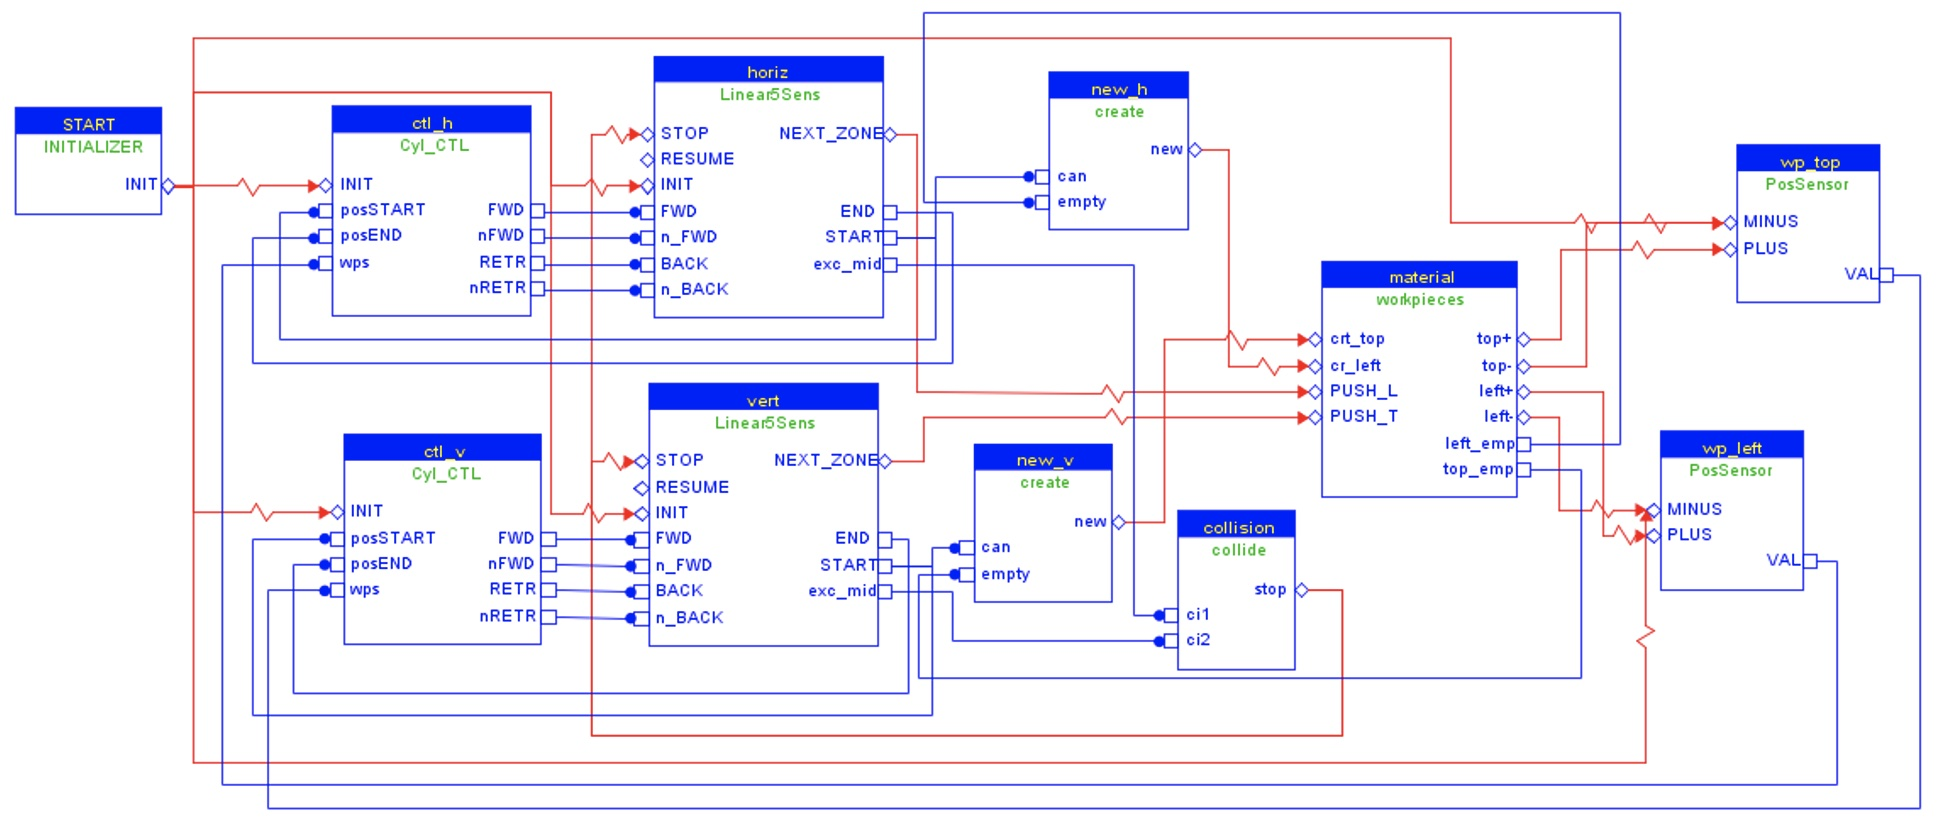
\includegraphics [width = .9 \textwidth] {images/nces_two_cylinders.jpg}
    \caption {NCES model of the two cylinders system.}
    \label {fig:nces_2_cyl}
\end {figure}

\VV{An abstract model of two processes interacting with each other with the help of buffer is presented in Fig.\ref{fig:nces_interprocess}. Here Process 1 adds a token to the Buffer, and Process 2 sees it and removes it from the buffer.}

\begin {figure}
    \centering
    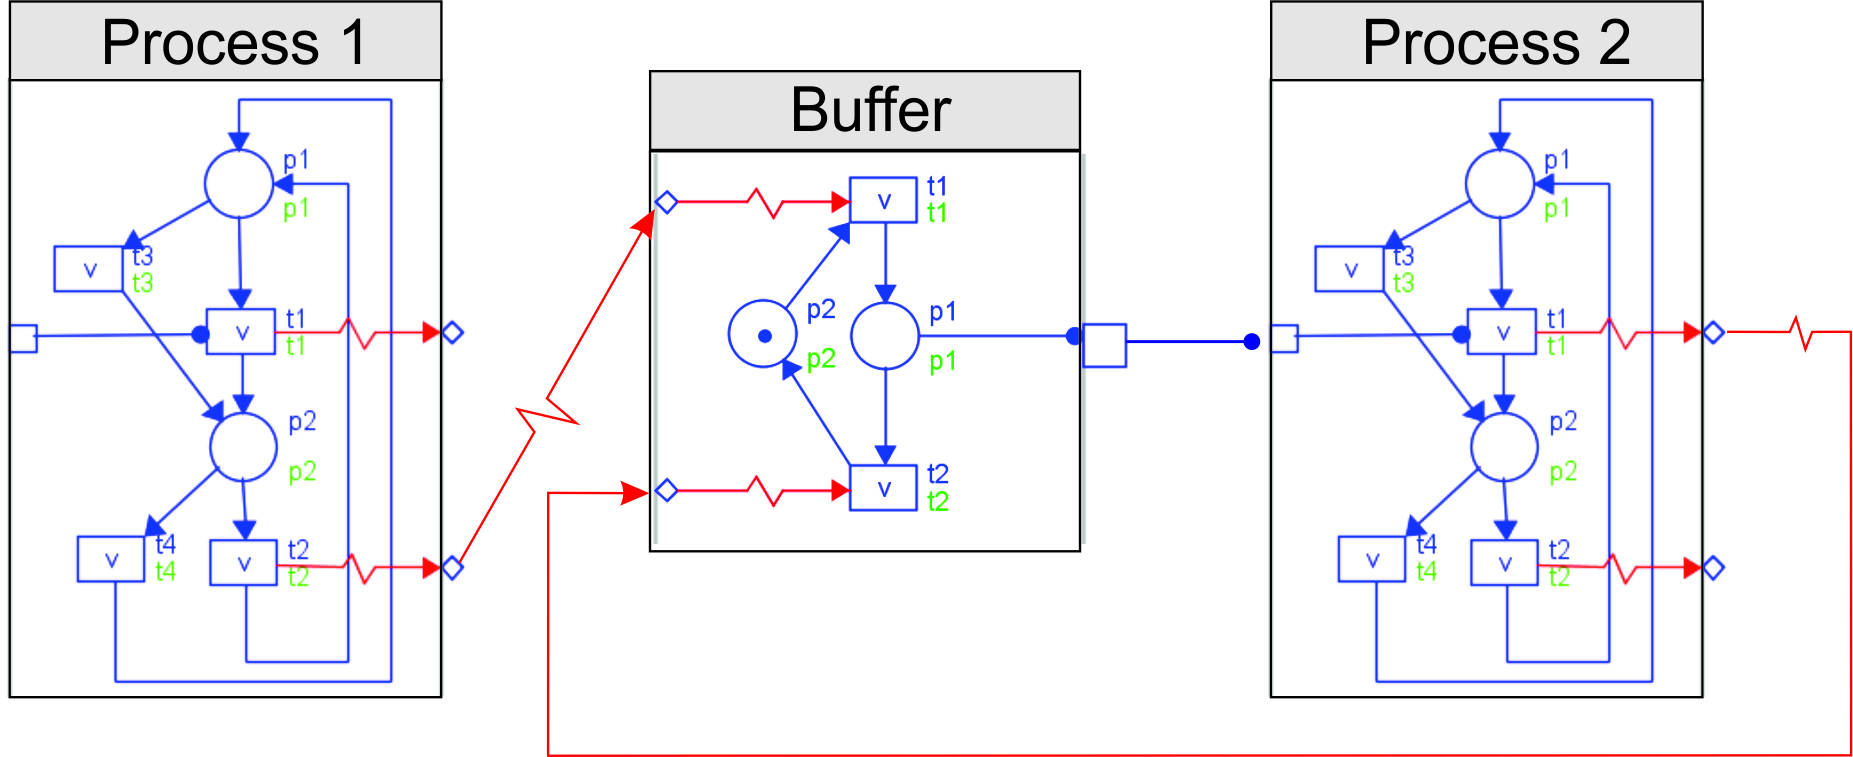
\includegraphics [width = .7 \textwidth] {images/interprocess.jpg}
    \caption {NCES model of interprocess communication.}
    \label {fig:nces_interprocess}
\end {figure}

\VV{A more sophisticated synchronous communication mechanism between clock-driven processes through a rendezvous channel} is modelled by means of NCES formalism in Fig. \ref{fig:rendezvous}. To verify the correctness of the channel’s operation the model-checking tool ViVe can be applied. The reachability graph of the model is presented in Fig.\ref{fig:verification}. 

\begin {figure}
    \centering
    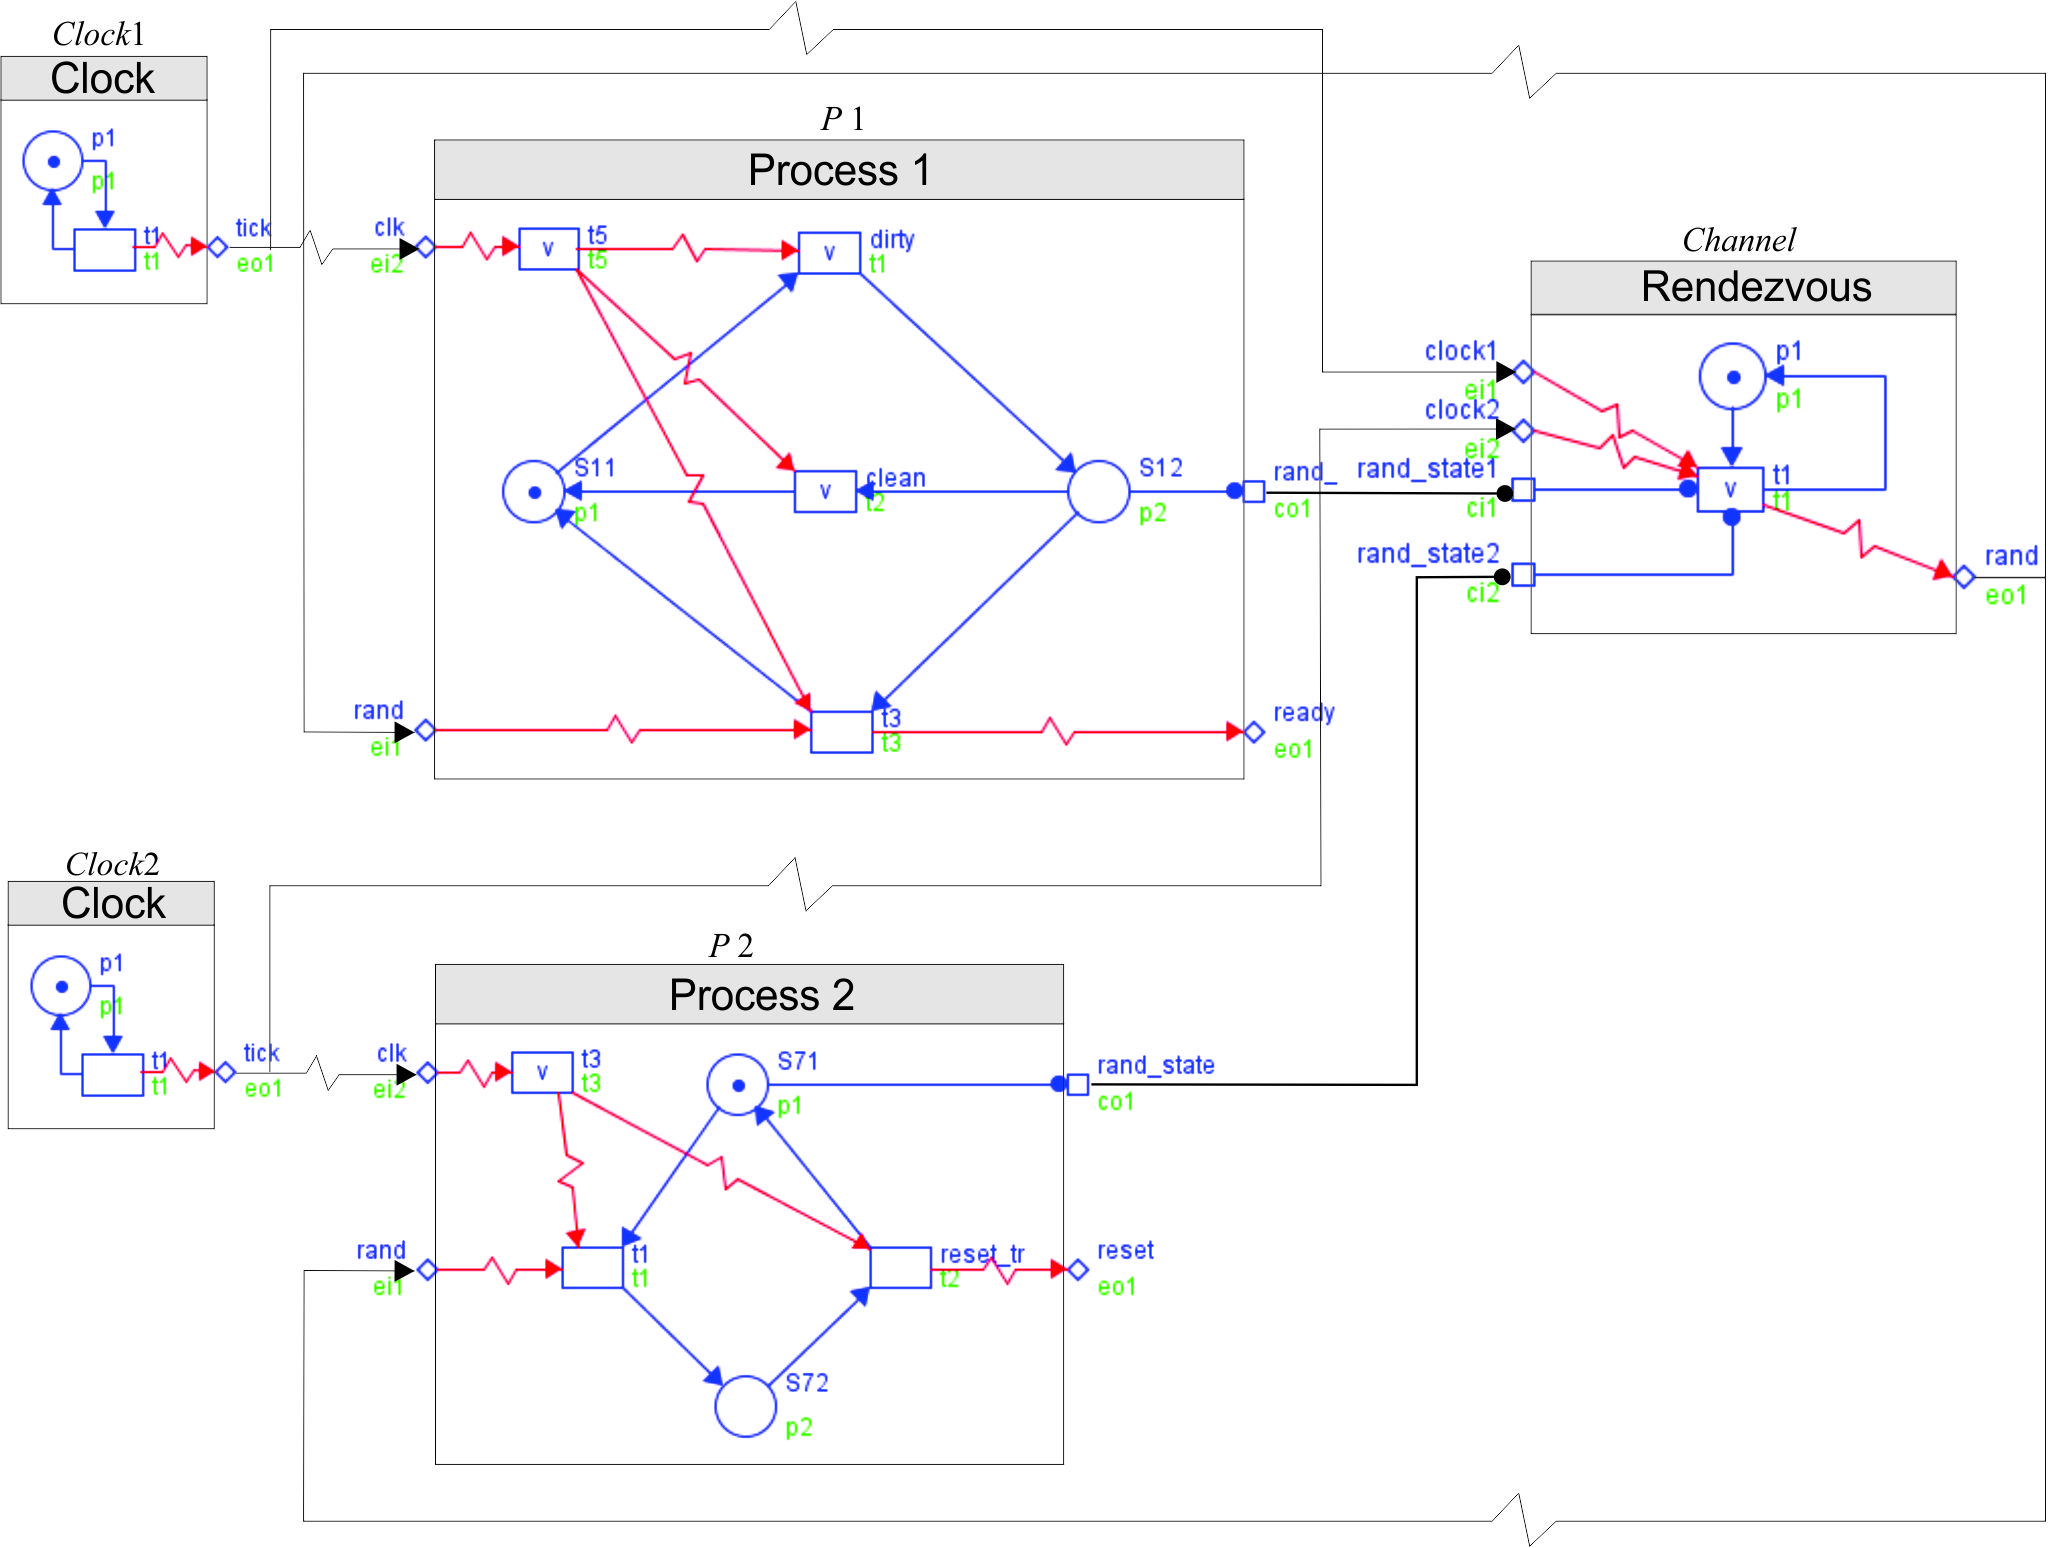
\includegraphics [width = .8 \textwidth] {images/rendezvous2.jpg}
    \caption {NCES model of the process synchronisation.}
    \label {fig:rendezvous}
\end {figure}


\begin {figure}
    \centering
    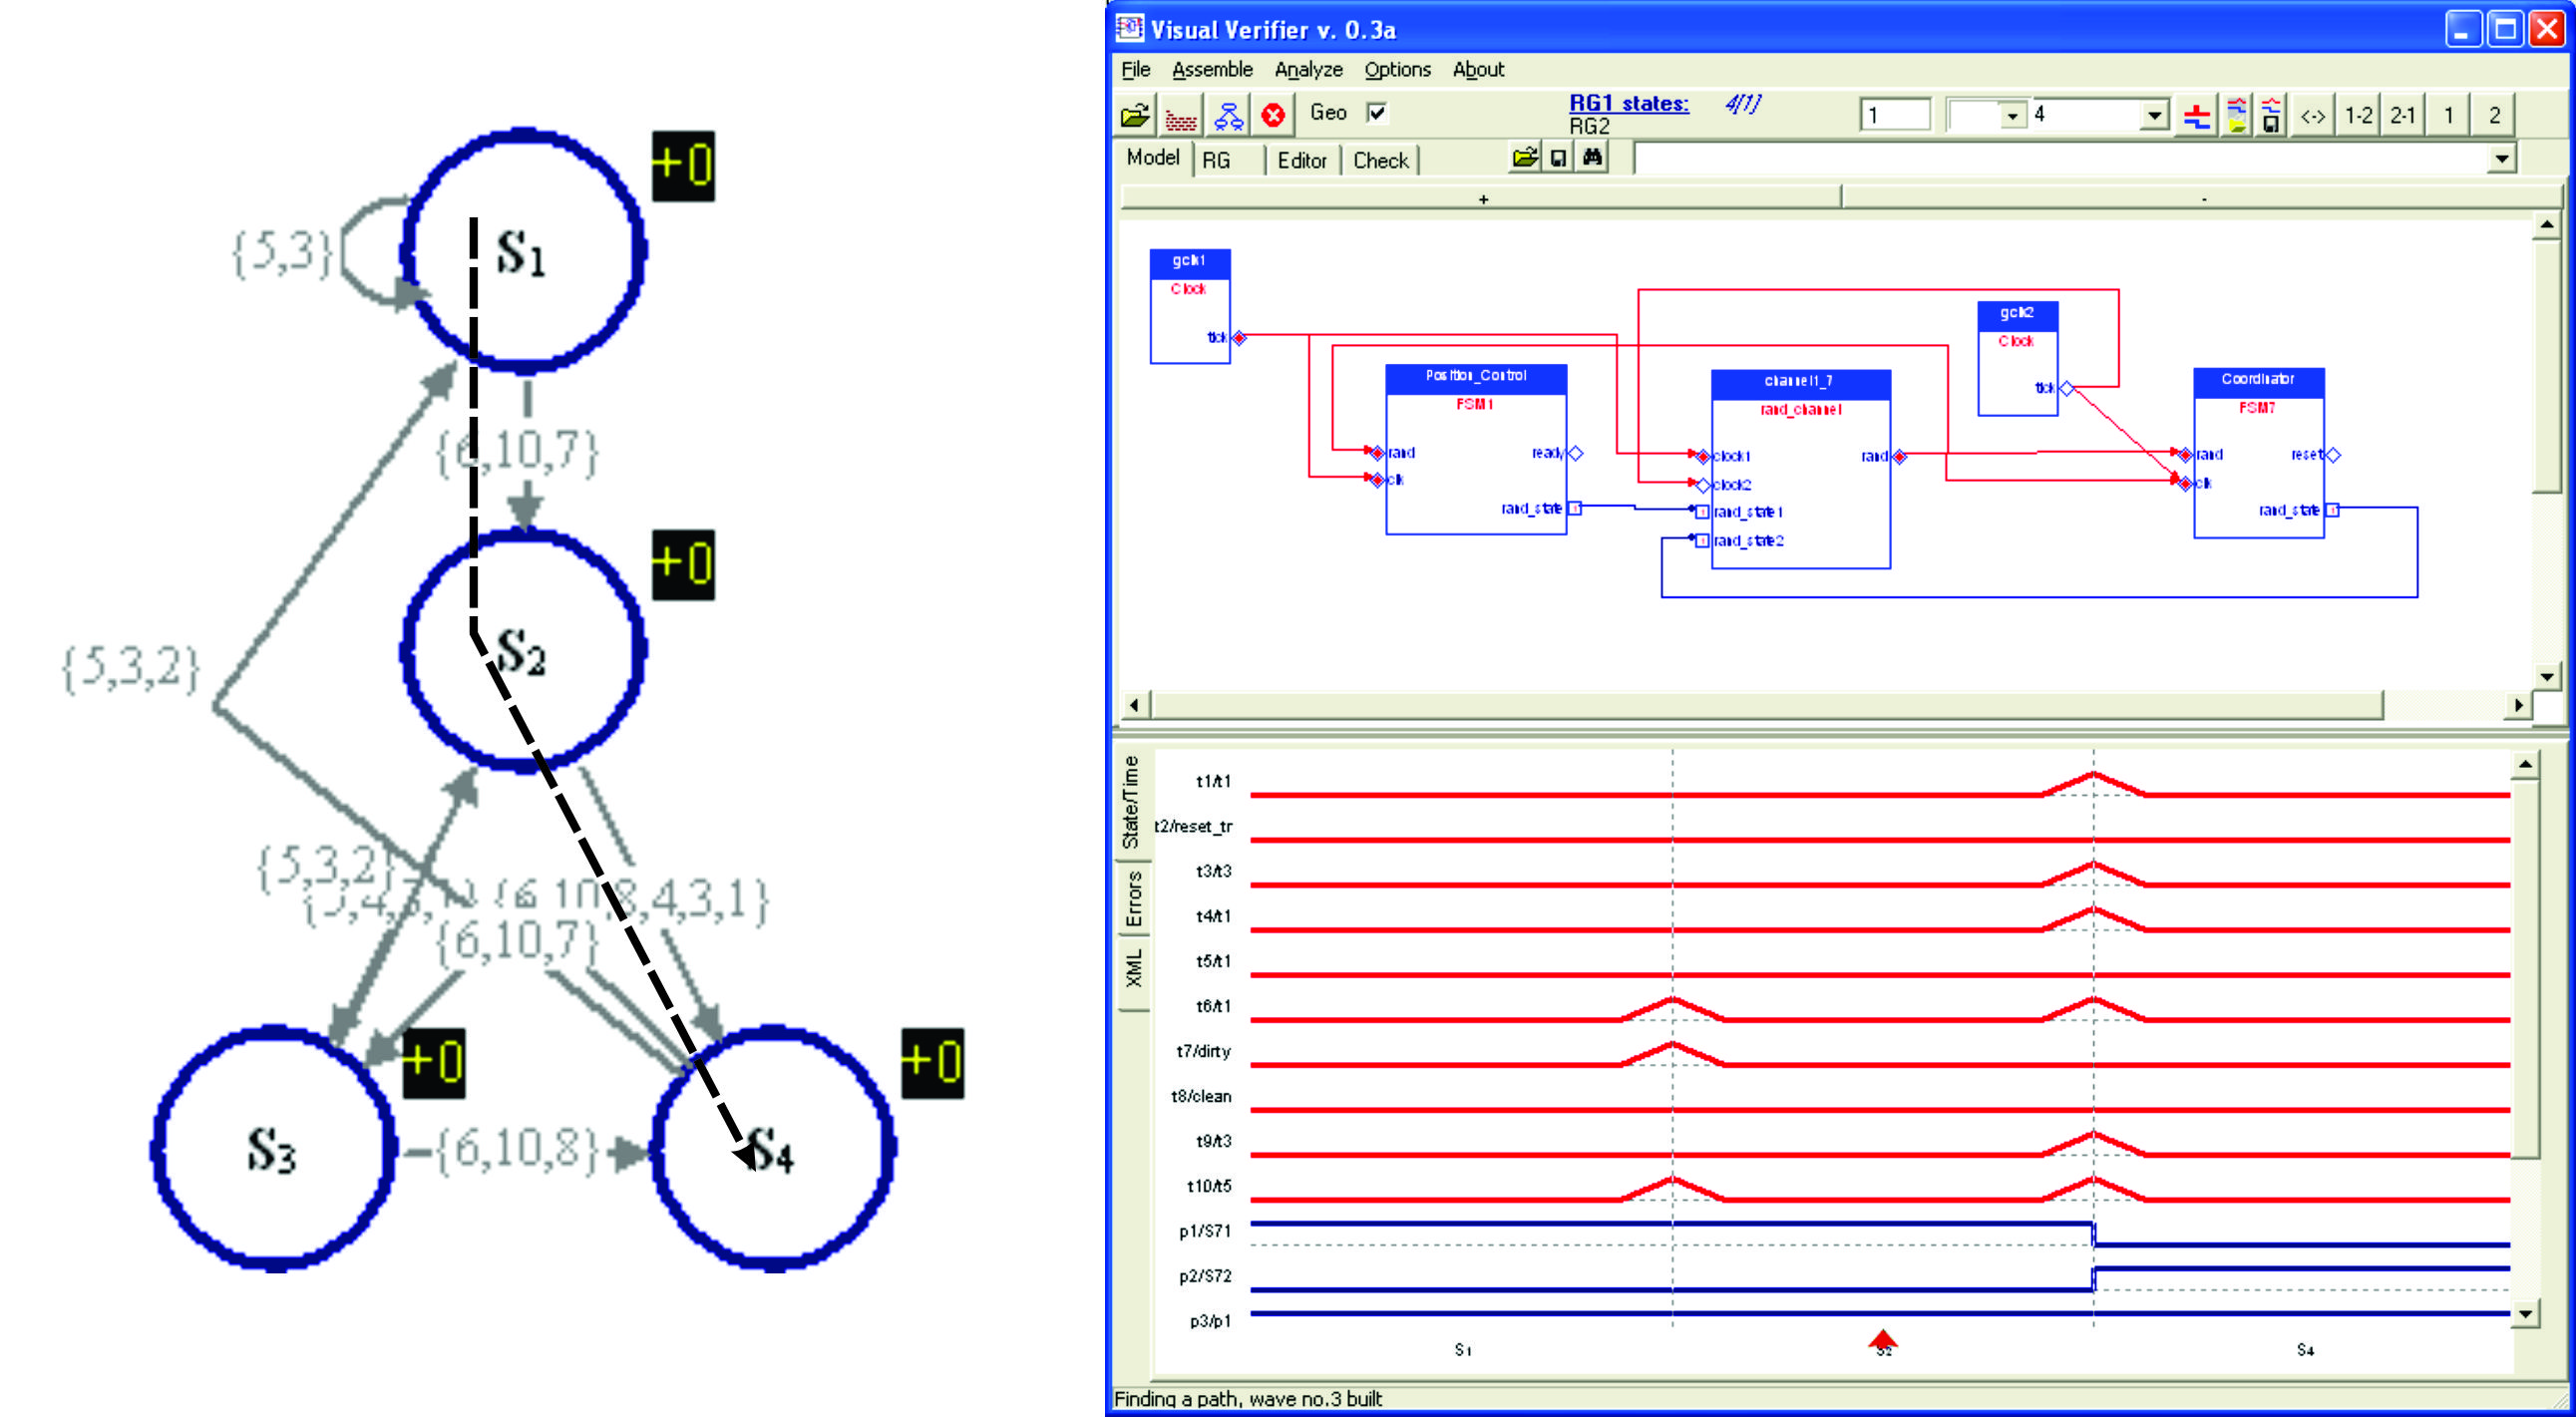
\includegraphics [width = .9 \textwidth] {images/verification.jpg}
    \caption {Reachability graph of the model (left) and the behaviour along the $S1\ra S2\ra S4$ trace (right), where the rendezvous occurs at the state transition  $S2\ra S4$.}
    \label {fig:verification}
\end {figure}

\section{IEC 61499 based modular engineering of automation systems}\label{sec:61499}

The {IEC 61499} architecture \cite{iec61499} is getting increasingly recognised as a powerful mechanism for engineering cyber-physical systems. 
In IEC 61499, the basic design construct is called function block (FB). Each FB consists of a graphical event-data interface and a set of executable functional specifications (algorithms), represented as a state machine (in basic FB), as a network of other FB instances (composite FB), or as a set of services (service interface FB). FBs can be interconnected into a network using event and data connections to specify the entire control application. The execution of an individual FB in the network is triggered by the events it receives. This well-defined event-data interface and the encapsulation of local data and control algorithms make each FB a reusable functional unit of software.


%A basic FB is defined by the signal interface (left-hand side) and also its internal state machine (called Execution Control Chart (ECC)) on the right-hand side, and the definition of algorithms executed in the ECC states.

A basic Function Block (FB)  consists of a signal interface (left-hand side) and an Execution Control Chart (ECC) state machine (right-hand side). The algorithms executed in the ECC states determine the behavior of the FB in response to changes in its inputs and its internal state.

A function block application is a network of FBs connected by event and data links as illustrated in the upper part of Fig. \ref{fig:similarity}, which illustrates models of the same one pneumatic cylinder system with IEC 61499 (top) and NCES (bottom). The structural similarity is supported by the semantic similarity since both modelling languages are event-based. Connections between modules in both modelling languages are passing events and data. 
This simplifies the modelling of IEC 61499 with NCES and several modelling and analysis tools were developed to explore it. 

\begin {figure}
    \centering
    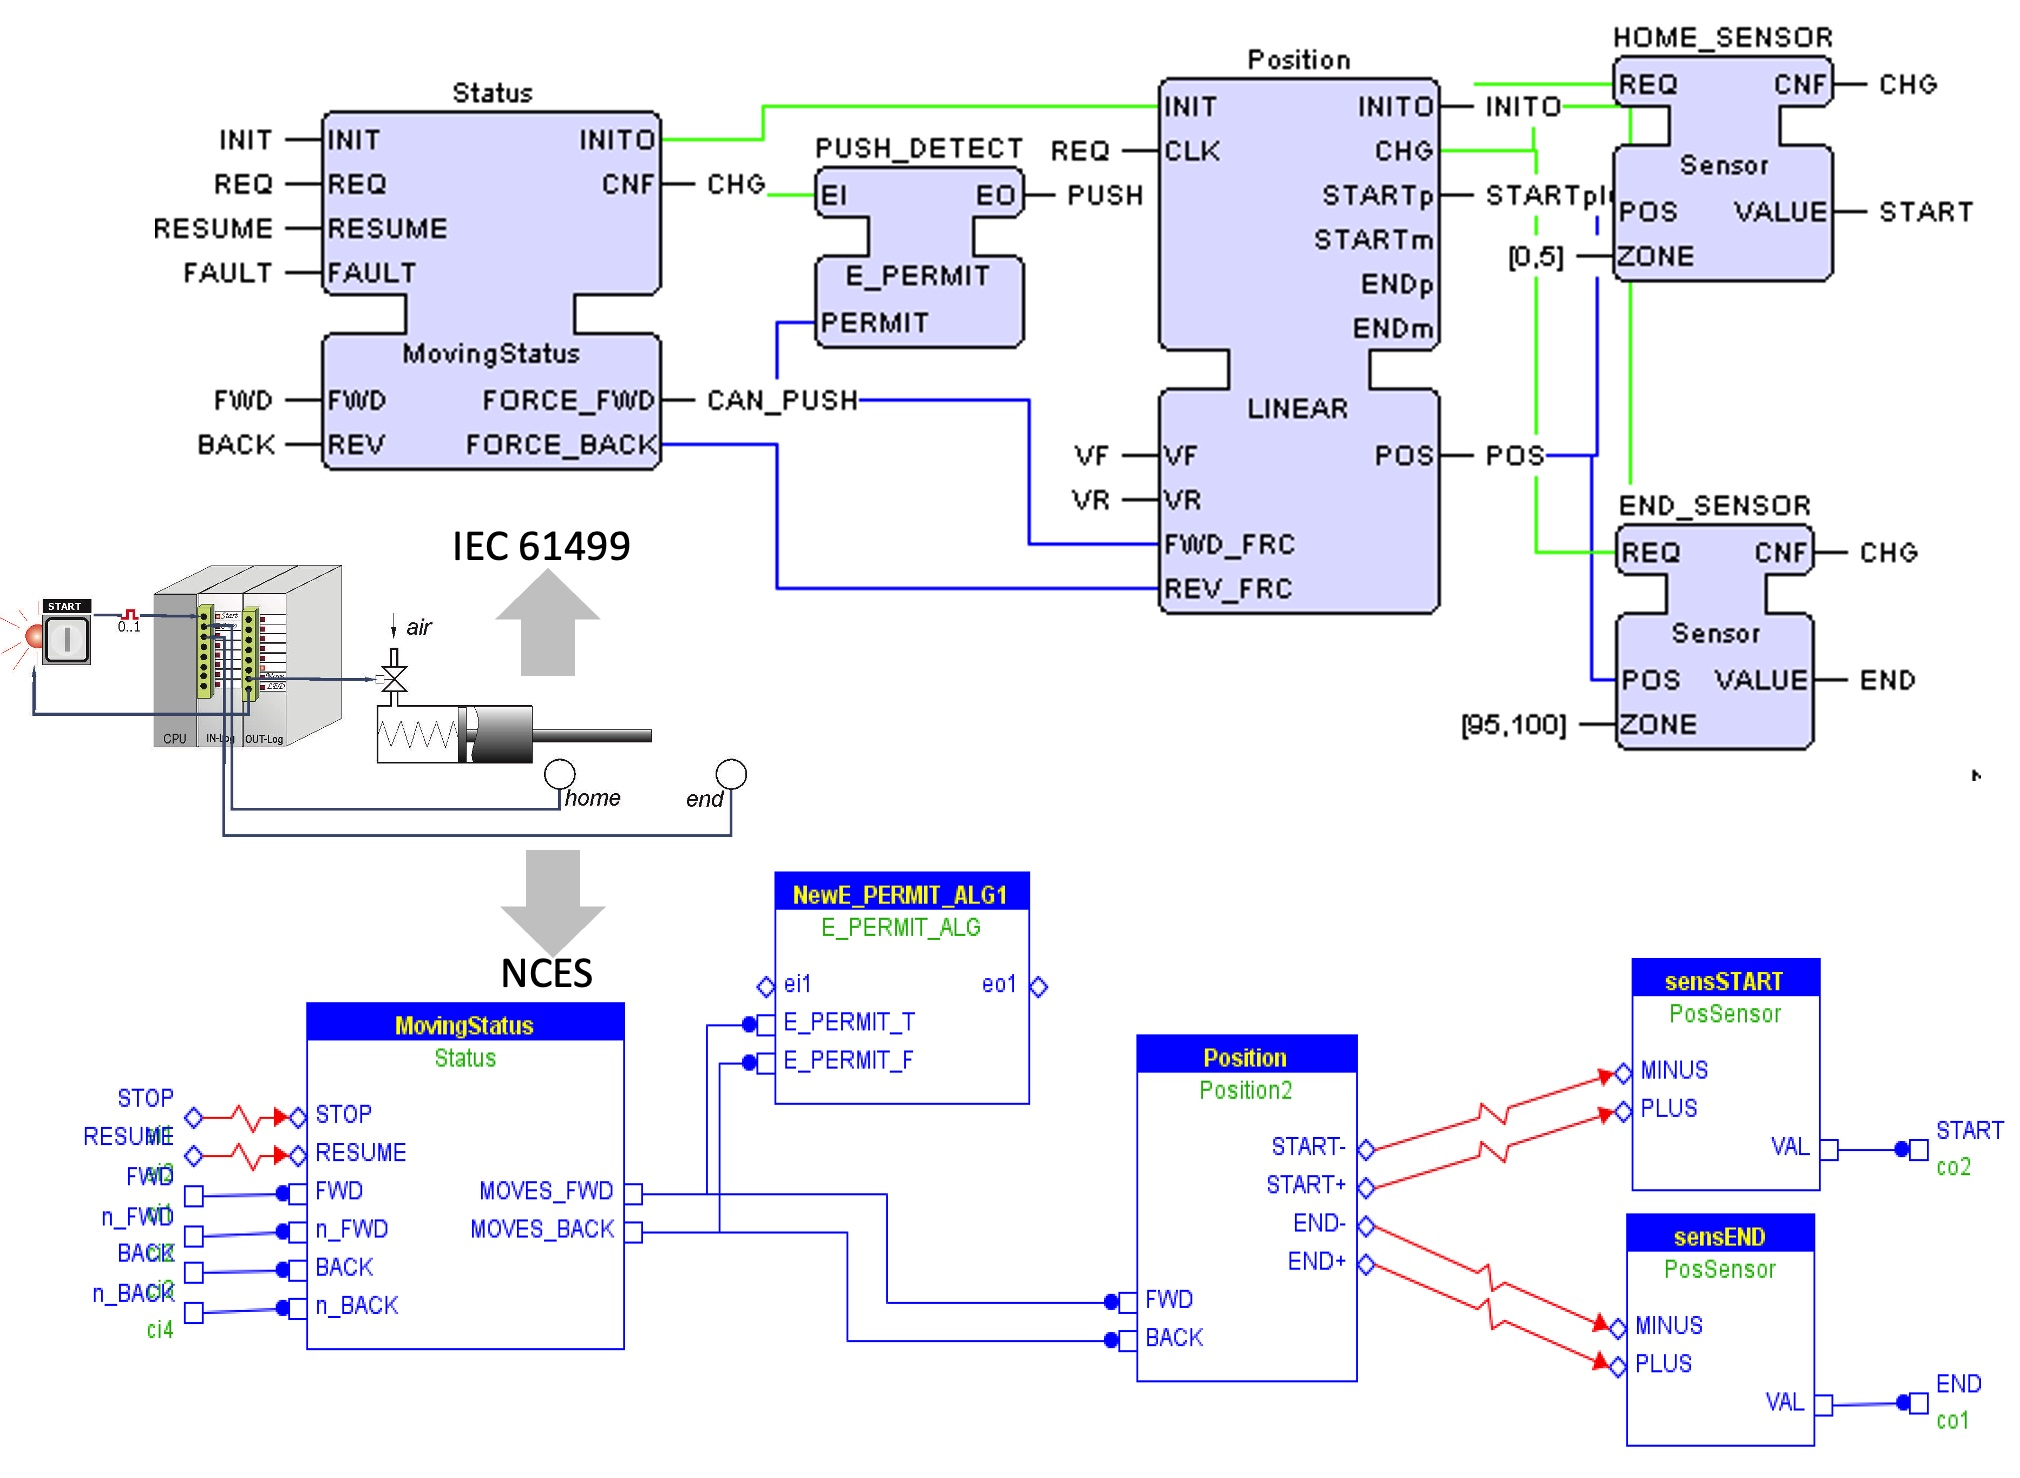
\includegraphics [width = .8 \textwidth] {images/similarity.jpg}
    \caption {Similarity of IEC 61499 and NCES models.}
    \label {fig:similarity}
\end {figure}

In 1998, way before the IEC 61499 was formally accepted as a standard by IEC, using an early draft, Hans-Michael Hanisch observed this stunning similarity and wrote a research proposal together with Peter Starke, supported by the German Research Council (DFG), on formal verification of IEC 61499 applications by means of NCES. That gave rise to a number of developments summarised in \cite{hanisch2009one}.

In particular, in 2001, Vyatkin and Hanisch developed a software package called "Verification Environment for Distributed Applications" (VEDA) for model-based simulation and verification \cite{vyatkin2001formal}. NCES is used for modelling and IEC 61499 function blocks are automatically converted with the help of VEDA for efficient simulation and verification. 

But, surprisingly, the NCES-IEC 61499 similarity helped develop a modelling approach in which IEC 61499 itself was directly used as a modelling language as it will be illustrated in Section \ref{sec:framework}. 

\section{Survey of works on modular engineering and modelling}\label{sec:survey}

To put the above-referenced developments on NCES and IEC 61499 to the broader context, in this section we present a brief survey of other related works on formal modelling and analysis of modular automation systems. 

\subsection{Modelling of flexible reconfigurable systems}

Reconfigurable Manufacturing Systems (RMS) are flexible and adaptable to manufacture various products to meet changing market demands. Meng \etal explain how complex RMS can be hierarchically modularized for modelling reconfigurability using coloured Object Oriented Petri nets \cite{MENG201081}. The  RMS model is developed with the help of the macro-level Petri net and the changes in RMS drive the change in Petri net.

Later,  Wu \etal introduced Intelligent Token Petri Net (ITPN) for modelling reconfigurable Automated Manufacturing Systems (AMS) \cite{wu2011intelligent}. The ITPN model captures dynamic changes in the system and the deadlock-free policy makes the model always deadlock-free and reversible. The change in configuration modifies only changed part of the current model and the deadlock-free policy remains the same.

In real-time systems temporal constants are inevitable and these systems need to be modelled to ensure that it satisfies functional and non-functional requirements. Recently, Kaid \etal developed  Intelligent Colored Token Petri Net (ICTPN) and it models dynamic changes in a modular manner and produces a compact model which ensures PN behavioural properties like boundness, liveness and reversibility but the ITCPN model lacks a conversion method to industrial control languages.

Reconfigurable Discrete Event System (RDES) such as reconfigurable manufacturing systems (RMS) has the ability to change the configuration of the system to adapt to changes in conditions and requirements.
Reconfigurable discrete event control systems  (RDECS) are an important part of RDESs.  Reconfiguration done at the run time is called Dynamic reconfiguration and it should occur without influencing the working environment and with no deadlock. Zhang \etal introduced the reconfiguration based on the Timed Net Condition/Event system (R-TNCES) and it is a formalism for the modelling and verification of RDECSs. SESA model checker does the layer-by-layer verification of R-TNCES \cite{zhang2013r}.  

Modern manufacturing systems switch energy-intensive machines between working and idle mode with the help of dynamic reconfiguration to save energy. The later works of Zhang \etal developed how formal modelling and verification of reconfigurable and energy-efficient manufacturing systems can be done using R-TNCES formalism and SESA tool is applied to check functional, temporal and energy efficient properties \cite{zhang2015modeling,zhang2018simulation}.

System reconfiguration in run-time is inevitable and a discrete event system with dynamic reconfigurability is called (DRDES). NCES is widely applied in DRDESs in the past decade. NCES are a modular extension of PN and it is used for modelling, analysis and control of DRDES. Many researchers worked on the modelling, analysis and verification of reconfigurable RMS. 

The system reconfiguration should be completed before the permissible reconfiguration delay. Whenever a reconfiguration event is triggered then DRDES should be able to go to the target state within the permissible reconfiguration delay otherwise it should reject the reconfiguration requirement. Zhang \etal developed to compute a shortest legal firing sequence (SLFS) of an NCES using Integer Linear Programming (ILP) under a given maximum permissible reconfiguration delay \cite{zhang2018shortest}.

Interpreted time Petri net (ITPN) is used to model real-time systems, which helps to increase the modelling power and expressiveness compared to (Timed Petri net) TPN's. Hadjidj \etal proposed  RT-studio (Real-time studio) for  modelling, simulation and automatic verification. \cite{hadjidj2013rt}. RT-studio tries to tighten the gap with the UPPAAL model checker by modularizing the ITPN model.  

Dehnert \etal introduced a new probabilistic model checker \cite{dehnert2017storm, hensel2022probabilistic} called Storm that can analyze both discrete- and continuous-time variants of Markov chains and Markov decision processes  (MDPs), using the Prism and JANI modelling languages, probabilistic programs, dynamic fault trees and generalized stochastic Petri nets. It has a flexible design that allows for easy exchange of solvers and symbolic engines, and it offers a Python API for rapid prototyping. Benchmark experiments have shown that Storm has competitive performance.

\subsection{Modelling of IEC 61499}\label{sec:mod61499}

Another approach to verify the application of IEC 61499 was presented by Schnakenhourg \etal, who explained the method to verify IEC 61499 function blocks by converting to the SIGNAL model \cite{schnakenbourg2002towards}. The specification also converts to a SIGNAL model and verifies using SILDEX from the TNI society.

In order to formally model function blocks in IEC 61499, it is necessary to first define their complete execution semantics. The semantic ambiguities in IEC 61499, can lead to different interpretations of function blocks. To address this, the Sequential Hypothesis can be used, which defines a more intuitive and clear sequential execution model of function blocks. Pang \etal \cite{pang2007towards},  developed IEC 61499 basic function  blocks using the sequential hypothesis, which assumes that blocks within a network are activated sequentially. They used NCES and verified the behaviour of the model using model-checking tools such as iMATCH and SESA. They later proposed a model generator \cite{pang2008automatic} that automatically translates IEC 61499 function blocks into the NCES formal model for the purpose of verification. The function blocks developed using the FBDK (Function Block Development Kit) are translated into functionally and semantically equivalent NCES models following the sequential execution model. This NCES model can be opened in ViEd and properties are verified using the ViVe tool.

%IEC 61499 is a standard for industrial control systems that aims to make applications portable in different runtime environments. 

Cengic \etal \cite{cengic2006formal} introduced a new runtime environment called Fuber, which uses a formal execution model to make the behaviour of IEC 61499 applications deterministic and predictable. They developed a tool to translate IEC 61499 function blocks into a set of finite-state automata and used the Supremica tool for supervisor verification and synthesis. After that, they  introduced a software tool to automatically generate formal closed-loop system models between control code and process models expressed as IEC 61499 function blocks, using extended finite automata (EFA) and Supremica for formal verification \cite{vcengic2008control}. They further extended this by defining the buffered sequential execution model (BSEM) and its formal verification using Supremica by analyzing the EFA model \cite{cengic2008definition}. In another study, Yoong \etal developed a tool to translate IEC 61499 function blocks to Esterel for verification \cite{yoong2010verifying}.  Existing verification tools for Esterel help to analyze the safety properties of IEC 61499 function block programs.

Formal verification of embedded control systems using closed-loop plant-controller models is becoming more popular.  However, the use of non-determinism in the model of the plant can lead to the complexity explosion in the model-checking process and make it difficult to verify the correctness of the plant model itself before it can be used in the closed-loop verification process. The paper \cite{patil2011closed} describes the integration of modelling principles into the Veridemo toolchain, and it also explains the implementation of controlled non-determinism in NCES systems. The controlled non-determinism limits the state space and eventually results in better verification times. This approach provides better model-checking performance with ViVe and SESA compared to NuSMV and UPPAAL model checkers with fully deterministic state machines. Later they introduced \cite{patil2015counterexample}  a framework for model checking and counter-example playback in simulation models used to verify the system. The control logic and dynamics of the plant are modelled using Net Condition/Event Systems formalism and ViVe/SESA toolchain is used for model checking. The counter examples for failures during model checking are played back in simulation models for a better understanding of the failures.



\begin{comment}

Wenbin William Dai et al \cite{dai2014configurable} proposes a configurable cloud-based validation environment for interoperability tests between various distributed automation systems using a multi-layer structure. The testing environment aims to provide automated configurable compliance testing at all levels and is designed with the use of the visual programming tool for the IEC 61499 standard, which is deployed remotely as a cloud-based service.



In this paper \cite{lindgren2015formal}, the authors focus on the Execution Control Chart semantics of the IEC 61499 standard for distributed control applications, to establish a well-formedness criterion that ensures a finite number of Execution Control Chart transitions for each triggering event. They also describe the first step towards the mechanization of the well-formedness checking algorithm in the Coq proof-assistant, so that the algorithm can be directly incorporated in a certified toolchain for analysis, compilation, and execution of IEC 61499 models.  A proof of concept prototype tool RTFM-4FUN has been developed to perform well-formedness checks on Basic Function Blocks using the extracted algorithm's code.
\end{comment}


The IEC 61499 standard is used for the development of distributed control systems, but it has limited support for reconfigurable architectures. To address this limitation, Guellouz \etal  proposed a new model called reconfigurable function blocks (RFBs) in their study \cite{guellouz2016reconfigurable}. They use GR-TNCES, a derivative of NCES, to model the system and applied the proposed approach to a medical platform called BROS. Further studies \cite{guellouz2018designing, fkaier2021modeling} proposed translating RFBs to GR-TNCES in order to verify their correctness and alleviate state space explosion in model checking. Additionally, the latter paper aimed to analyze probabilistic properties and used a smart-grid system as a case study to demonstrate the approach. The study also developed a visual environment called ZiZo v3 for modelling reconfigurable distributed systems.

 The formal verification technique is a reliable approach to ensure the correctness of instrumentation and control (I\&C) systems. It mentions that model-checking is widely used in avionics, the automotive industry, and nuclear power plants but has some  difficulties in locating errors in the model. The Oeritte tool, presented in the first study of Ovsiannikova \etal \cite{ovsiannikova2021oeritte}, is a solution for assisting analysts in the debugging process of formal models of instrumentation and control systems. It uses a method for automatic visual counterexample explanation and includes reasoning for both the falsified LTL formula and the NuSMV function block diagram of the formal model of the system. The tool addresses the challenges of counterexample visualization, LTL formulae, and counterexample explanation by providing methods, visual elements, and user interface. The second study,\cite{ovsiannikova2021towards}, presents the development of a model-checking plugin for IEC 61499 systems in the FBME graphical development environment. The plugin automates the process of converting the system to a formal model, model-checking, and providing a visual explanation of counterexamples.

 The next step to verification is the formal synthesis of correct-by-design systems with ensured safe operation. Missal and Hanisch \cite{missal2008modularA,missal2008modularB} present a modular synthesis approach. It is based on the modular backward search in order to avoid the complexity of generating all states and state transitions of the plant model.
It uses modular backward steps that describe the trajectories leading to forbidden states. The generation of these trajectories is stopped as soon as a preventable step is found. From this information, the models of the controllers are generated. 
Each controller has decision functions and communications functions. Together they establish a network of local, interacting controllers with communication. It is assumed that the plant is completely observable, i.e. the local controllers have complete information about the local states of the partial plants they are supposed to control. 
The paper also contributes with the definition of the behaviour of the plant without its complete composition. This means that the behaviour can be studied by means of modular steps within the modules and their interaction across module boundaries.

Dubinin \etal in \cite{dubinin2015synthesis} demonstrate safety controller synthesis  using the description of the plant and forbidden behaviour, proposing a method of synthesis of adaptive safety controller models for distributed control systems based on reverse safe Net Condition/Event Systems (RsNCES). The method allows for the generation of prohibiting rules to prevent the movement of closed-loop systems to forbidden states. The method is based on a backward search in the state space of the model.

\section{Use IEC 61499 for Condition/Event Modelling: A Comprehensive Tool Chain} \label{sec:framework}

%\begin {figure}
%    \centering
 %   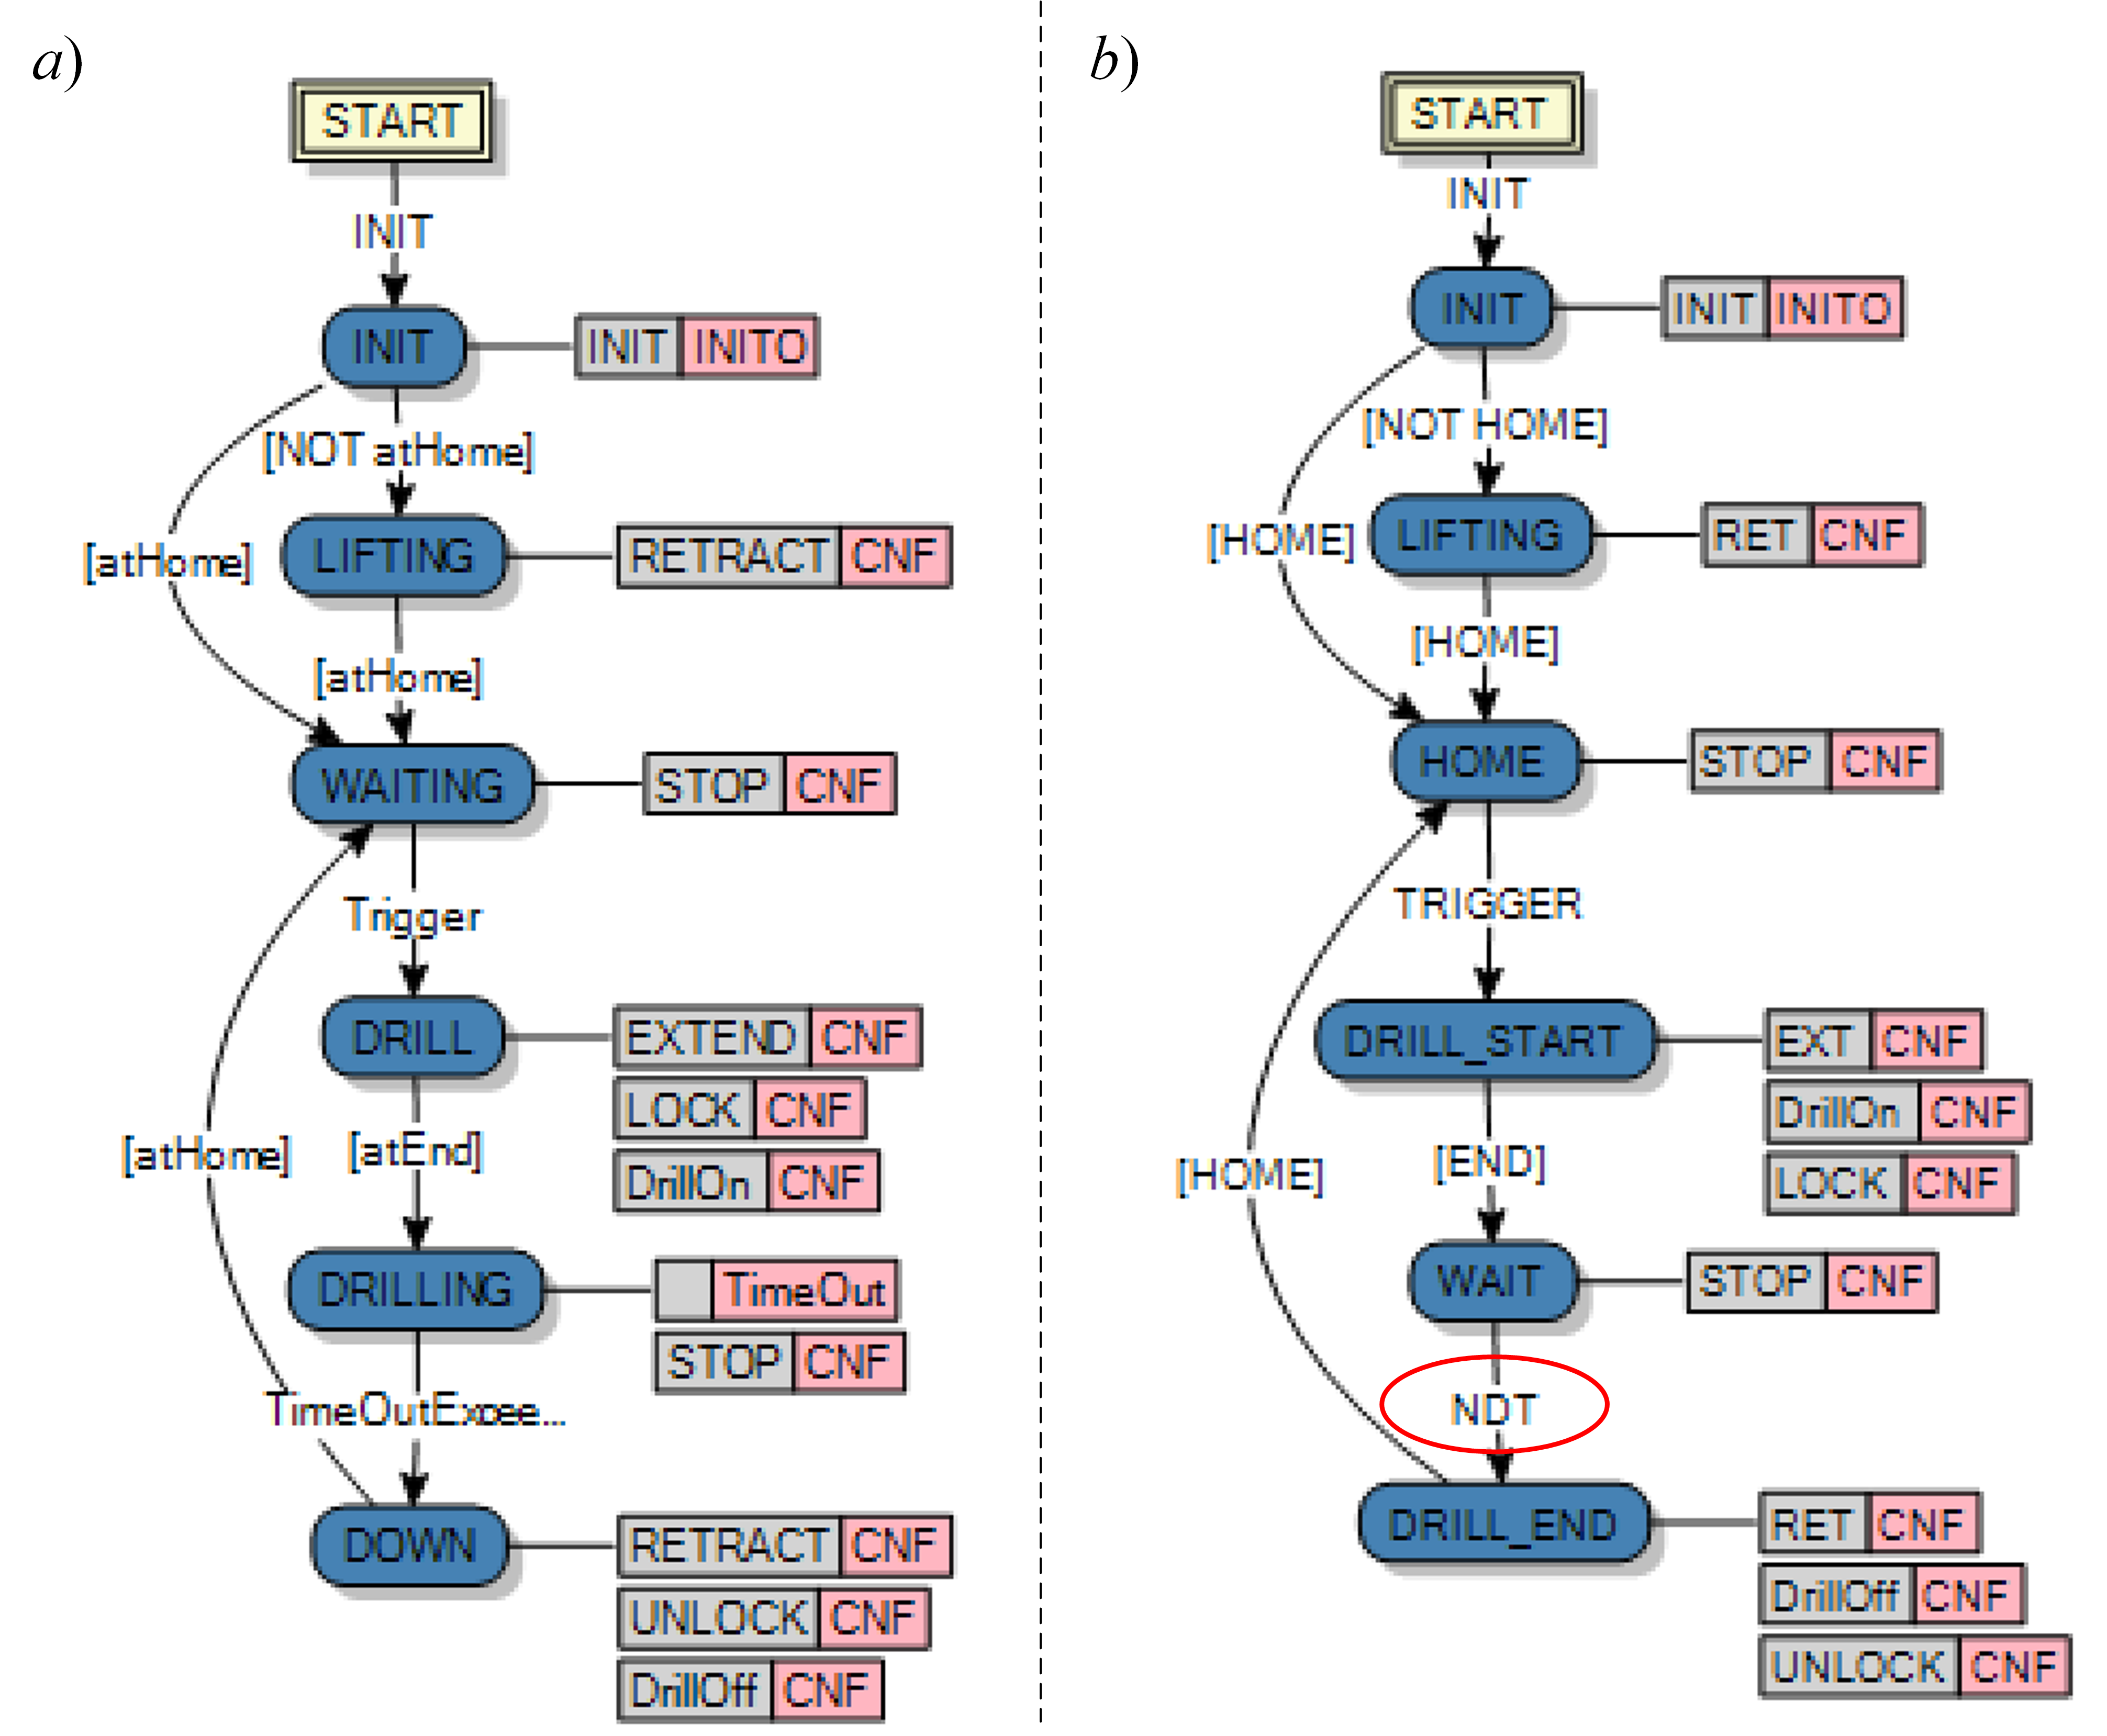
\includegraphics [width = .5 \textwidth] {images/Fig10.png}
 %   \caption {a) The ECC of the real drill controller; b) The ECC of the modified drill controller with a non-deterministic transition modelling the time delay.}
 %   \label {fig:NDT_Controller}
%\end {figure}

The works on formal modelling and verification of IEC 61499 systems by means of NCES and its analysis tools have confirmed the benefits of exploring their structural and semantic similarities. On the other hand, applying the verification to systems of industrial scale has raised several questions:
\begin{itemize}
\item Model-checking tools for NCES require constant support and improvement, which was lacking. A bridge to industrially supported powerful tools was desirable.
\item Verification should be a part of the regular engineering and testing process that includes testing by simulation, and analysis of results. 
\end{itemize}
 
 %Formal verification, specifically model-checking is a method of proving or disproving an algorithm with respect to a specification or property. It is computationally demanding but has been successfully used in other areas of computer systems engineering and can be an efficient way to prove the correctness of safety-critical applications. 
 
 Towards the first goal, Patil \etal \cite{patil2015formal} introduce a method for formally modelling and verifying IEC 61499 function blocks, a component model used in distributed embedded control system design, using the Abstract State Machines (ASM) as an intermediate model and the SMV model checker. The ASM model is translated into the input format of the SMV model checker, which is used to formally verify the properties. The proposed verification framework enables the formal verification of the IEC 61499 control systems, and also highlights other uses of verification such as the portability of IEC 61499-based control applications across different implementation platforms compliant with the IEC 61499 standard. Their other work \cite{patil2015neutralizing} proposes a general approach for neutralizing semantic ambiguities in the IEC 61499 standard by the formal description of the standard in ASM.



Another study \cite{patil2015formal}, highlights the importance of formally verifying function block applications in different execution semantics and the benefits of verifying the portability of component-based control applications across different platforms compliant with the IEC 61499 standard. The paper applies the formal model to an example IEC 61499 application and compares the verification results of the two-stage synchronous execution model with the earlier cyclic execution model, to verify the portability of the IEC 61499 applications across different platforms.

After that, they addressed the SMV modelling of the IEC 61499 specific timer function block types, particularly in hierarchical function block systems with timers located at different levels of hierarchy \cite{drozdov2016formal}. The paper also introduces plant abstraction techniques to reduce the complexity of cyber-physical systems models using discrete-timed state machine models implemented in UPPAAL. The approach is demonstrated with an example of formal verification of a modular mechatronic automated system and is shown to extend the abilities in the validation of real cyber-physical automation systems. A toolchain was developed to support the described modelling method, including an automatic FB-to-SMV converter for the transformation of IEC 61499 FB applications to the control part of SMV models. This approach can be used for the verification of newly developing industrial safety-critical systems such as smart grids.

Addressing the second goal, the road map on the creation of a tool-chain connecting engineering with verification seamlessly was outlined in  \cite{vyatkin2008closed}.  A problem-oriented notation within the IEC 61499 syntax for creating formal closed-loop models of cyber-physical automation systems \cite{xavier2021cyber} is proposed. The notation enables the creation of a comprehensive toolchain for the design, simulation, formal verification, and distributed deployment of automation software. The toolchain includes an IEC 61499-compliant engineering environment, a converter for functions blocks to SMV code, the NuSMV model-checker and utilities for interpreting counterexamples. The proposed method aims to overcome the hurdle of verifying and analyzing function blocks implemented in IEC 61499 standard by providing a toolchain for continuous development and testing of distributed control systems. 



\begin {figure*}
    \centering
    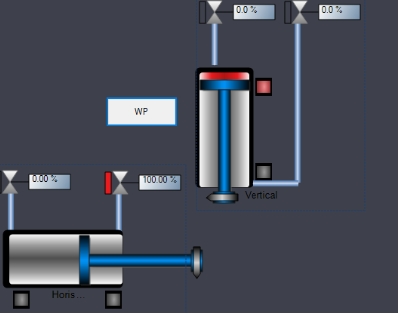
\includegraphics [width = 0.5 \textwidth] {images/Two_Cylinder.PNG}
    \caption {Visualisation of the Two Cylinder system produced by the model of the plant implemented in IEC 61499.}
    \label {fig:two_cylinder_HMI}
\end {figure*}

The two-cylinder system  consists of two orthogonal pneumatic cylinders controlled by a switch button shown in figure \ref{fig:two_cylinder_HMI}. It is built using five basic function blocks, including a controller function block (Button FB) that triggers the movement of the cylinders when pressed, plant function blocks (HorCyl and VerCyl FBs) that model the physical device of each cylinder, and controller function blocks (HorCTL FB and VerCTL FB) that control the plant by analyzing sensor signals and triggering actuator signals. These blocks receive information from the switch FB and send orders to the plant FB.





\begin {figure*}
    \centering
    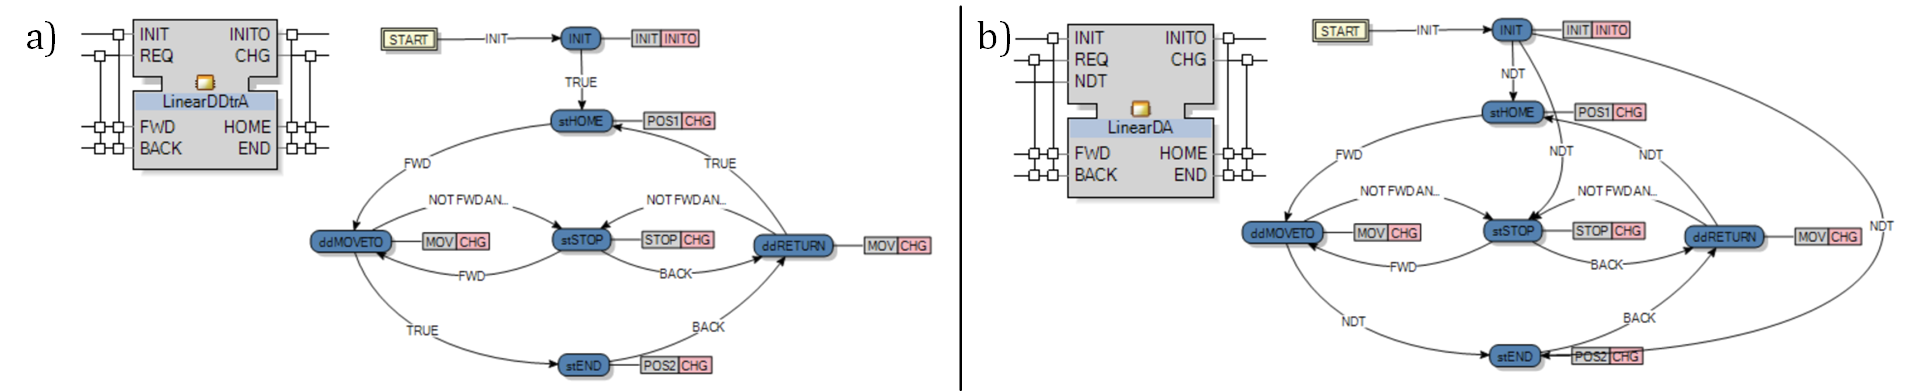
\includegraphics [width = 1 \textwidth] {images/NDT_linear.PNG}
    \caption {a) Deterministic discrete state linear motion process model without NDT, b) Discrete state linear motion process model with NDT.}
    \label {fig:NDT_in_Plant}
\end {figure*}

To implement the closed-loop approach to system modelling, the model of the plant needs also to be modelled using function blocks. A discrete state linear motion of a cylinder for a linear motion, for example, a linear axis, can be represented by a LinearDDtrA function block with two states (sHOME and sEND) that transition between them based on input signals (BACK or FWD) Fig. \ref{fig:NDT_in_Plant}, a. However, this minimal approach may not capture all possible errors that can occur during transitions between states. 

By using NDT (Non-deterministic transition), a more comprehensive model can be created by adding two dynamic states (ddMOVETO and ddRETURN) to capture potential errors during transitions Fig. \ref{fig:NDT_in_Plant},b.

The axis moves from the stHOME state to the stEND state via the motion state ddMOVETO when the FWD signal is TRUE. The use of NDT (Non-Deterministic Transition) in the transition from the ddMOVETO state to the stEND state models the unknown duration of the motion from one state to another. The NDT event input of the LinearDA function block, which was unassigned in the application, is reserved for non-deterministic transitions in the proposed modelling notation. This approach can provide a more detailed and accurate representation of the system, allowing for more thorough formal verification. 

The (multi-) closed-loop model of the two cylinders system using this extension of the IEC 61499 language is shown in Fig. \ref{fig:twocylindersfb}. This is nothing else, but a Condition/Event discrete-state model represented by means of IEC 61499. 

\begin {figure*}
    \centering
    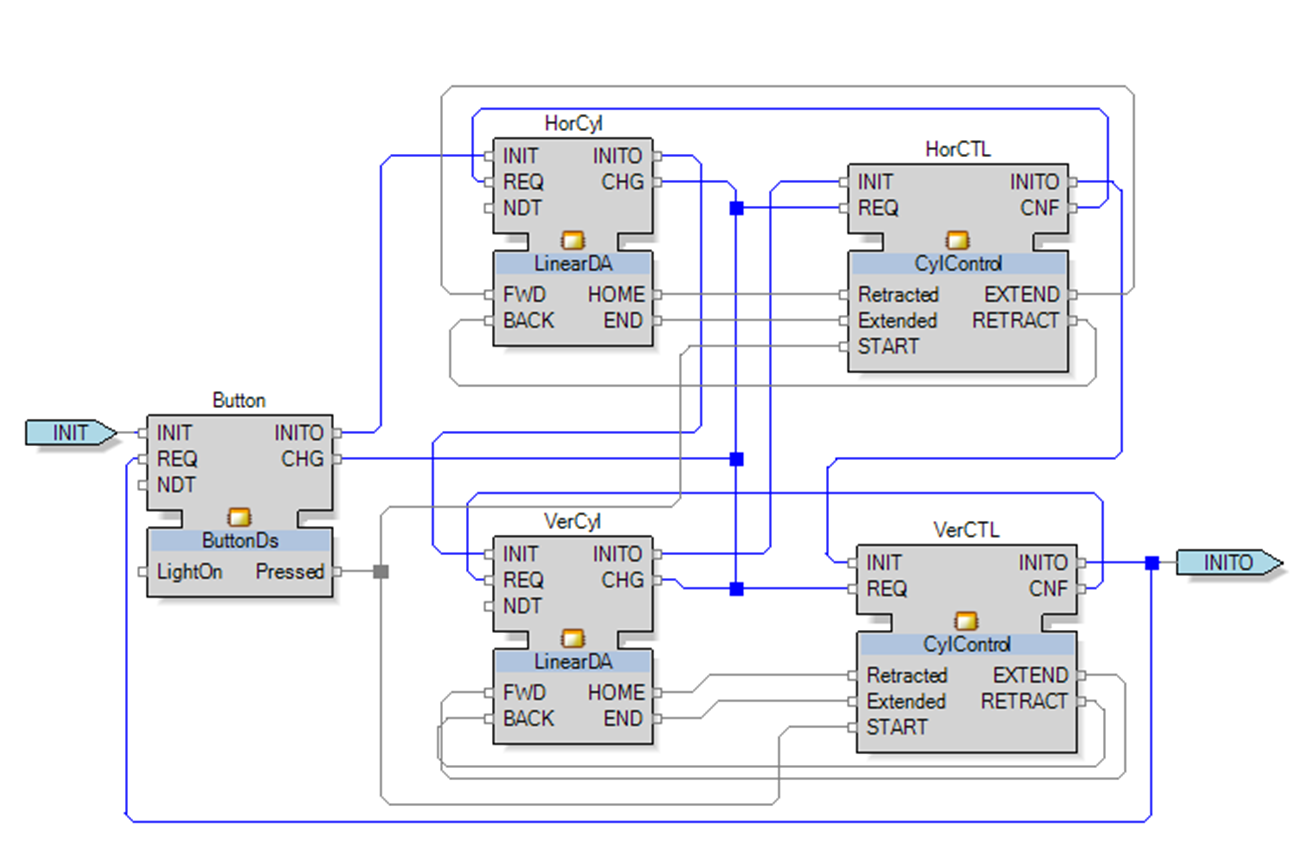
\includegraphics [width = 0.8 \textwidth] {images/twocylindersfb.PNG}
    \caption {Complete two cylinders model in the modified FB language.}
    \label {fig:twocylindersfb}
\end {figure*}

%Mapping of the NDT in SMV modelling will be described in a later section.

%Non-deterministic transition can be used to simplify controller models that contain timers. In a drill example, the drilling process needs to be done for different durations, which is achieved with a composite function block that includes a real controller and an E\_DELAY function block. Formal modeling of timers in SMV can be computationally difficult, but this complexity can be avoided by substituting the concrete delay duration with non-deterministic transitions using the NDT signal. By doing this, the controllers can be modified to reduce the complexity of model-checking. The execution control chart for the real drill controller and the modified drill controller are also provided \ref{fig:NDT_Controller}.




\begin{comment}
In SMV, non-deterministic choice can be achieved by providing a set of values to a signal. To accomplish this, designers can use two statements. The first statement is used to declare the variable NDT as a Boolean type, and the second statement is used to initialize the NDT variable to either TRUE or FALSE. This allows the signal to take on different values in each transition, providing the necessary non-determinism for formal verification.


\begin{lstlisting}[breaklines,basicstyle=\small]
1 | VAR NDT:= boolean;
2 | init(NDT):= { TRUE, FALSE };
\end{lstlisting}

By assigning a set of possible values to the NDT variable, in this case either TRUE or FALSE, and initializing it in every transition, it makes the NDT variable unpredictable in each transition. This allows for non-determinism in the model, which is useful for formal verification as it allows for the exploration of all possible behaviors of the system.

\begin{lstlisting}[breaklines,basicstyle=\small]
3 | next(NDT):={ TRUE, FALSE };
\end{lstlisting}

Implementing non-determinism in every transition can be limited by introducing conditions in the next statement. For example, if it is not necessary for the NDT variable to choose values in every transition, we can design the code in a way that the NDT variable only chooses values in certain transitions based on certain conditions. This can help to reduce the number of possible states and transitions, making the model more efficient and easier to analyze.
\begin{lstlisting}[breaklines,basicstyle=\small]
4 | next(NDT):= case
5 | 	Condition: { TRUE, FALSE };
6 |     TRUE : NDT;
7 | Esac;
\end{lstlisting}

\end{comment}

The fb2smv tool is a model generator that is used to generate SMV (Symbolic Model Verifier) models of function block systems in IEC 61499. It is part of a formal verification tool-chain that includes the model checker NuSMV and a tool for analyzing counterexamples in terms of the original FB system. The tool uses the Abstract State Machine (ASM) as an intermediate model to convert IEC 61499 function blocks expressed in XML format into a formal model. The generated SMV code has a structure that consists of a declaration part and an ASM rules part. The tool can convert both basic and composite function blocks, and also includes additional features such as limiting variable boundaries to reduce the state space, changing the execution order of FBs, and deciding the input event priority by changing its order. Additionally, the tool has been updated to include a proposed non-deterministic transitions notation.

Closed-loop modelling is a powerful approach for the verification of distributed industrial automation systems, as it allows for a comprehensive evaluation of the system's behaviour. However, it requires the creation of a model of the plant, which can be a complex and resource-intensive task, typically done manually. In these papers \cite{xavier2021plant,xavier2022process,xavier2022interactive,xavier2022plant}, authors show how to generate the plant and controller models automatically using a data-driven approach. The above-mentioned toolchain has been effectively used in these experiments to verify, simulate and analyse counterexamples. 


\section{Summary and Open Problems}\label{sec:summary}


Systems with dynamically created and terminated modules or dynamic connections between modules cannot be efficiently and naturally modelled within the C/ES paradigm and require complicated workarounds.

The idea of modular analysis of NCES has not been developed although the absence of token flow between the NCES modules could potentially facilitate it.

\begin {figure}
    \centering
    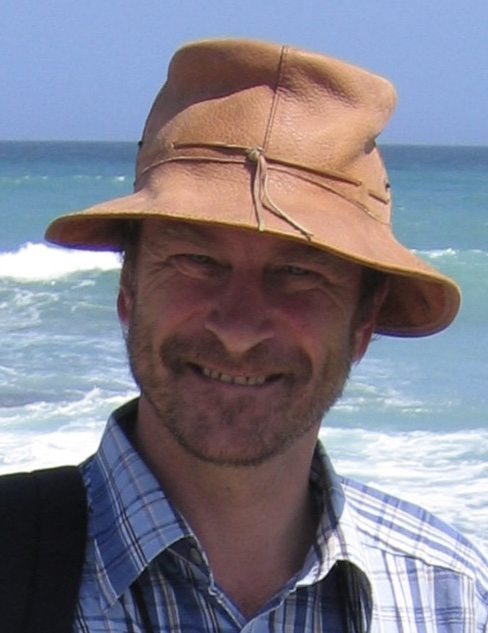
\includegraphics [width = .35 \textwidth] {images/Hanisch.jpg}
    \caption {Hans-Michael Hanisch (1957-2022).}
    \label {fig:Hanisch}
\end {figure}


\section*{Acknowledgments}
This paper attempts to be a tribute to Professor Hans-Michael Hanisch who has been a co-inventor and a great enthusiast and proponent of NCES as a part of the closed-loop modelling concept. 
 

%
%\begin{table}[!t]
%% increase table row spacing, adjust to taste
%\renewcommand{\arraystretch}{1.3}
% if using array.sty, it might be a good idea to tweak the value of
% \extrarowheight as needed to properly center the text within the cells
%\caption{An Example of a Table}
%\label{table_example}
%\centering
%% Some packages, such as MDW tools, offer better commands for making tables
%% than the plain LaTeX2e tabular which is used here.
%\begin{tabular}{|c||c|}
%\hline
%One & Two\\
%\hline
%Three & Four\\
%\hline
%\end{tabular}
%\end{table}





% conference papers do not normally have an appendix


% use section* for acknowledgment
% \section*{Acknowledgment} %%%%%%%%%%%%%%%%%%%%%%%%%%%%%%%%%%%%%%%%%%%%%%%%%%%%%%%%%%%%%%%%%%%%%%%%%


% The authors would like to thank...





% trigger a \newpage just before the given reference
% number - used to balance the columns on the last page
% adjust value as needed - may need to be readjusted if
% the document is modified later
%\IEEEtriggeratref{8}
% The "triggered" command can be changed if desired:
%\IEEEtriggercmd{\enlargethispage{-5in}}

% references section

% can use a bibliography generated by BibTeX as a .bbl file
% BibTeX documentation can be easily obtained at:
% http://mirror.ctan.org/biblio/bibtex/contrib/doc/
% The IEEEtran BibTeX style support page is at:
% http://www.michaelshell.org/tex/ieeetran/bibtex/
\bibliographystyle{splncs04}
% argument is your BibTeX string definitions and bibliography database(s)
\bibliography{sns,main}
%\bibliography{sns.bib}

%
% <OR> manually copy in the resultant .bbl file
% set second argument of \begin to the number of references
% (used to reserve space for the reference number labels box)
% \begin{thebibliography}{1}

% \bibitem{IEEEhowto:kopka}
% H.~Kopka and P.~W. Daly, \emph{A Guide to \LaTeX}, 3rd~ed.\hskip 1em plus
%   0.5em minus 0.4em\relax Harlow, England: Addison-Wesley, 1999.

% \end{thebibliography}




% that's all folks
\end{document}


